\section{Question 2}
Assume $\boldsymbol{r}_0$ and $\boldsymbol{v}_0$ as:


$$
\boldsymbol{r}_0 = \begin{bmatrix}
    1600 & 5310 & 3800
\end{bmatrix}^{\textrm{T}}_{km}, \quad
\boldsymbol{r}_0 = \begin{bmatrix}
    -7.350; & 0.4600 & 2.470
\end{bmatrix}^{\textrm{T}}_{km/\sec}
$$

\subsection{Part a}
the n-body problem was solved with MATLAB with the n-body function in the question directory.
The results are illustrated below.
\begin{figure}[H]
    \caption{3D trajectory}
    \centering
    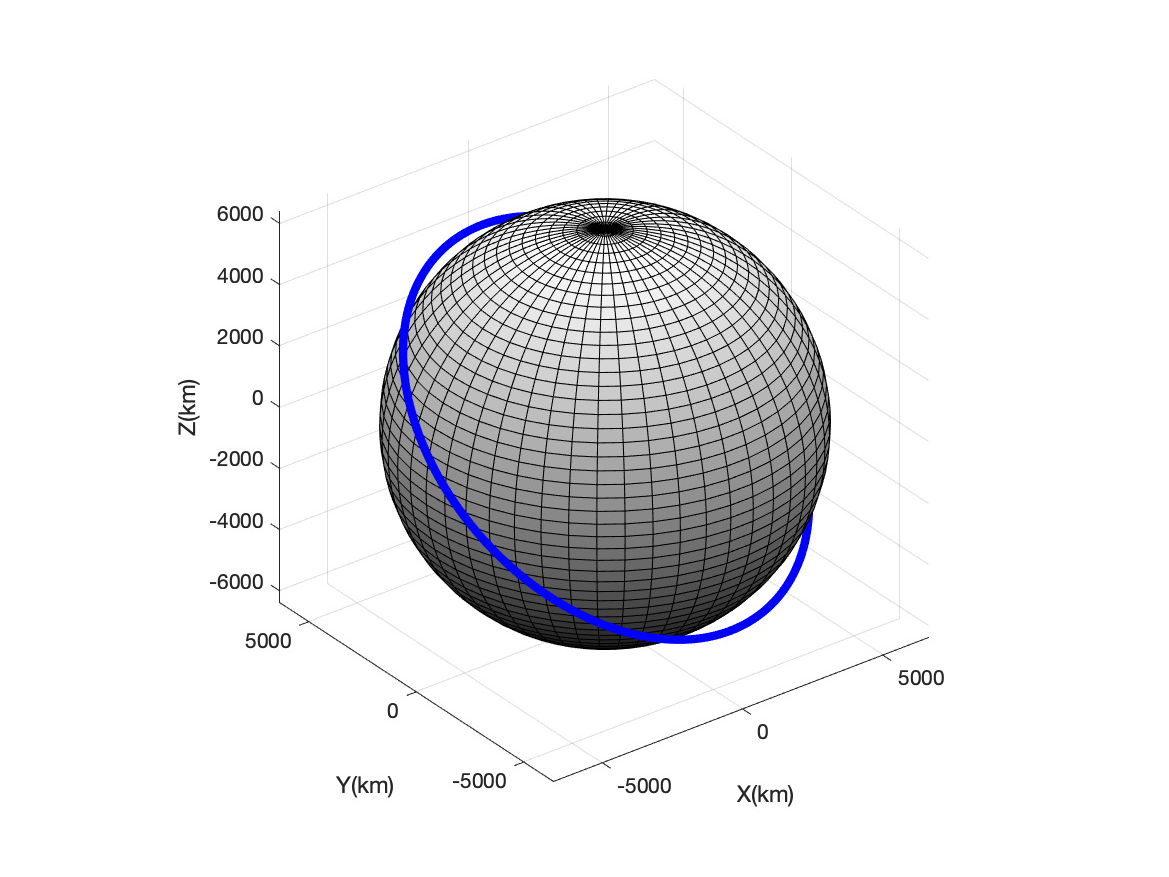
\includegraphics[width=16cm]{../Figure/Q2/3Dof_view}
\end{figure}

\begin{figure}[H]
    \caption{3D trajectory in zx axis}
    \centering
    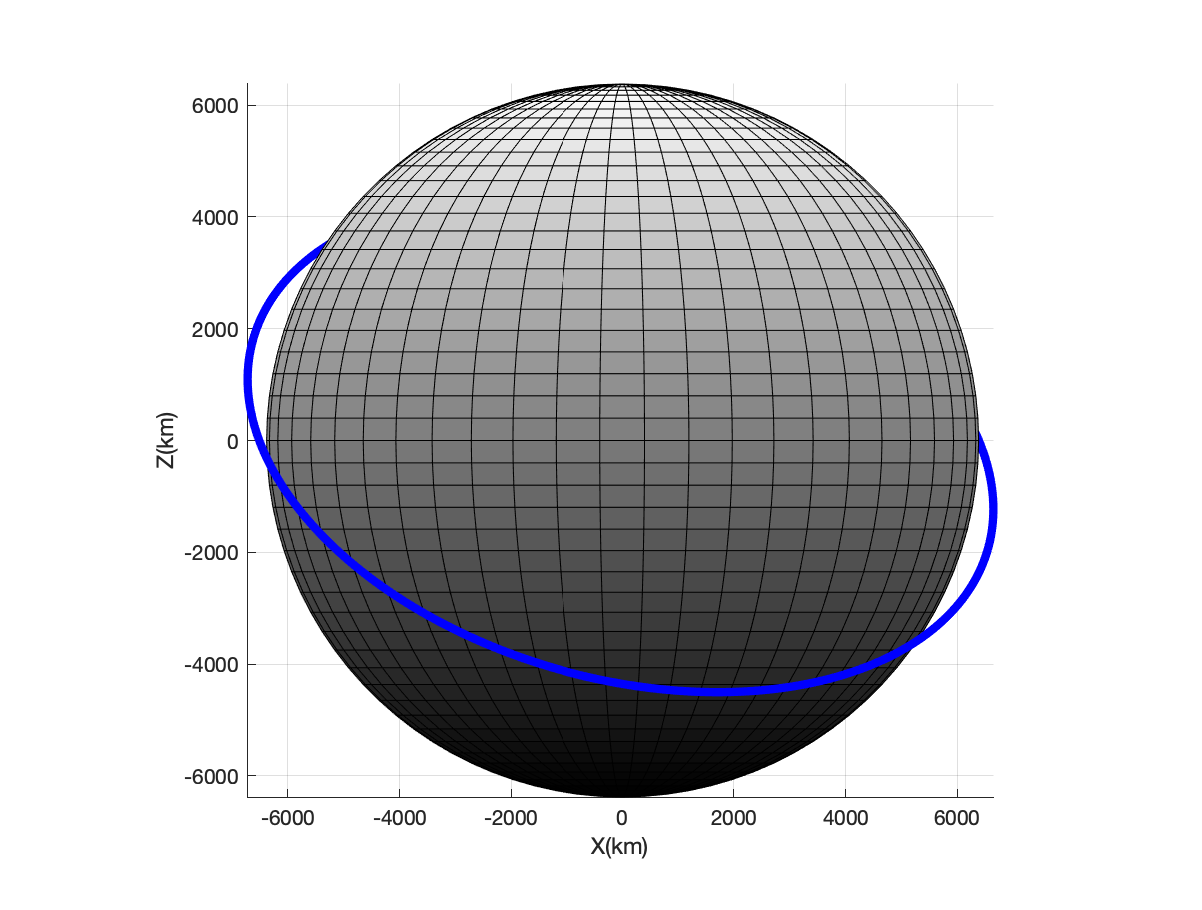
\includegraphics[width=16cm]{../Figure/Q2/xz_view}
\end{figure}

\begin{figure}[H]
    \caption{3D trajectory in zy axis}
    \centering
    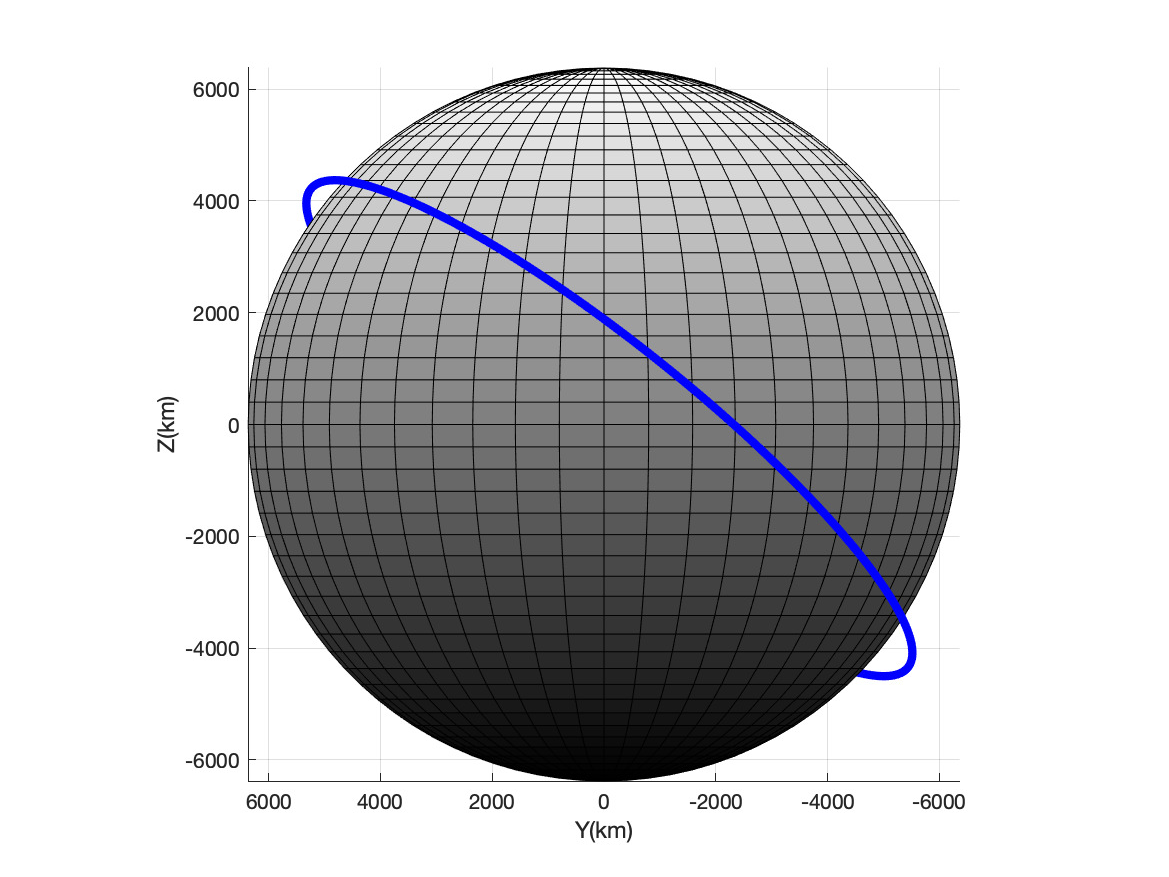
\includegraphics[width=16cm]{../Figure/Q2/yz_view}
\end{figure}

\begin{figure}[H]
    \caption{3D trajectory in xy axis}
    \centering
    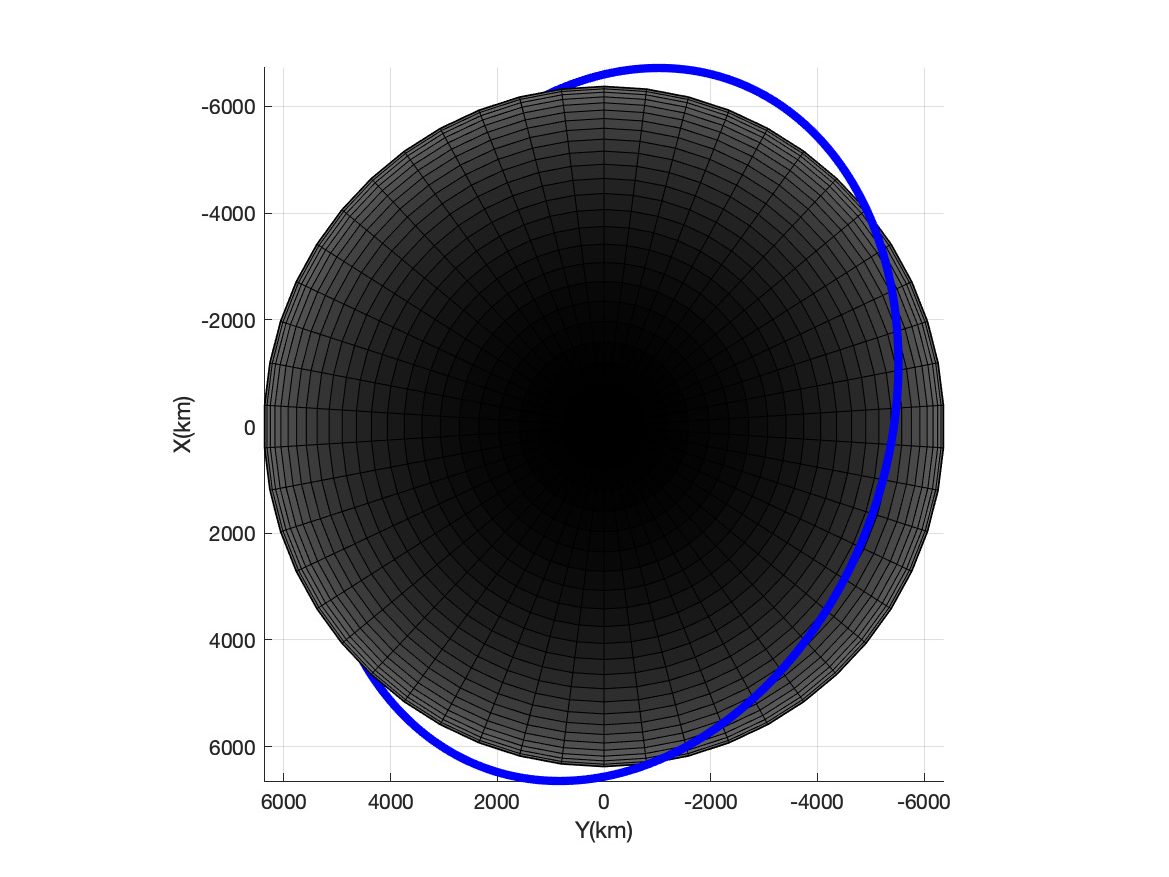
\includegraphics[width=16cm]{../Figure/Q2/xy_view}
\end{figure}

\subsection{Part b}

Using the below transfer matrix to transfer from ECI coordinate to the ECEF coordinate.
$$
\boldsymbol T^{ECCF-ECI} = \begin{bmatrix}
    \cos(\omega_Et) & -\sin(\omega_Et)& 0\\
    \sin(\omega_Et) &  \cos(\omega_Et)& 0\\
            0       &      0          & 1
\end{bmatrix}
$$

$$
\phi = \arccos(\dfrac{\boldsymbol r(3)}{r})
$$

$$
\lambda = 
\begin{cases}
\arctan(\dfrac{\boldsymbol r(1)}{r_{xy}}),& \boldsymbol r(2) > 0\\
2\pi-\arctan(\dfrac{\boldsymbol r(1)}{r_{xy}}),& \boldsymbol r(2) \leq 0\\
\end{cases}
$$

\begin{figure}[H]
    \caption{Satellite latitude versus its longitude for one day}
    \centering
    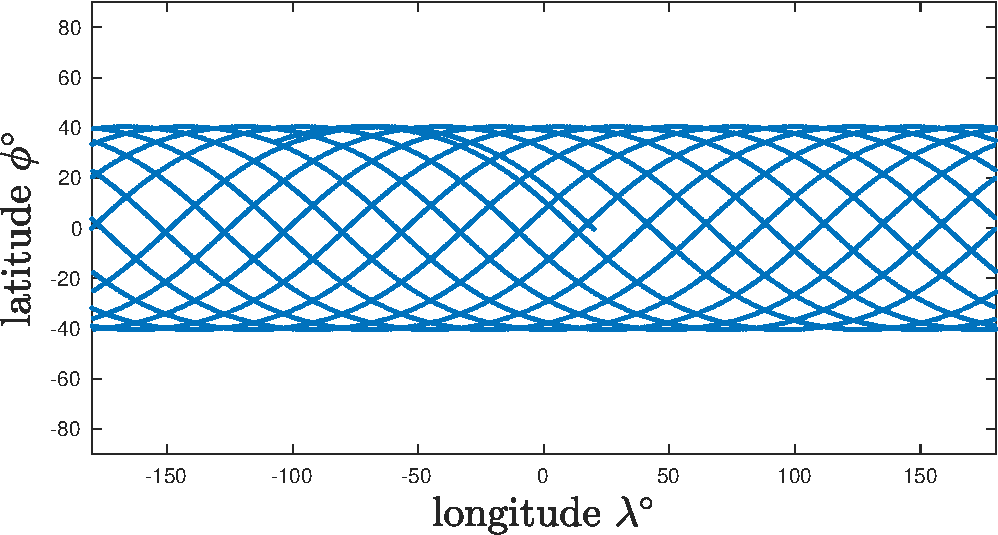
\includegraphics[width=16cm]{../Figure/Q2/latlong}
\end{figure}

Below the figure drawn provided by tamaskis, please click \href{https://github.com/tamaskis/ground_track-MATLAB}{here} to see the source code. Please use the mentioned library to run code or skip the part on earth fig.

\begin{figure}[H]
    \caption{Satellite latitude versus its longitude for one day}
    \centering
    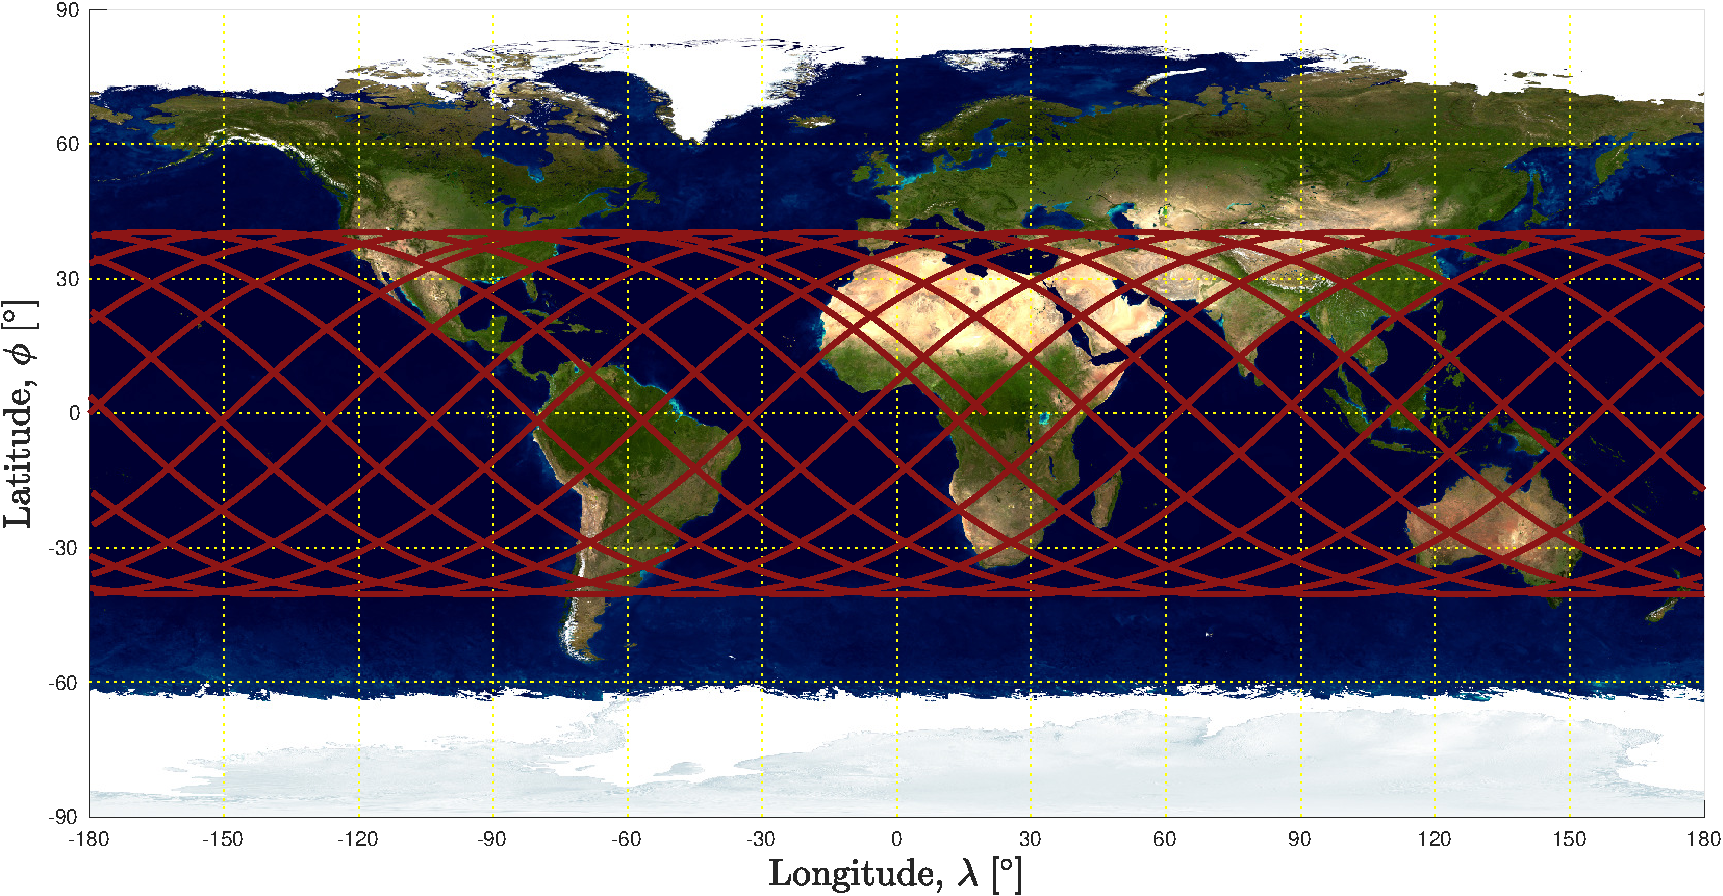
\includegraphics[width=16cm]{../Figure/Q2/latlong_earth}
\end{figure}

\subsection{Part c (Bonus)}

In this section find the orbital elements, then, change the inclination to $0.4_{rad}$ (using oe2ecf and vec2orbElem functions). Then, find $\boldsymbol{r}_0$ and $\boldsymbol{v}_0$ by new orbital elements.
The results are illustrated below.
\begin{figure}[H]
    \caption{3D trajectory}
    \centering
    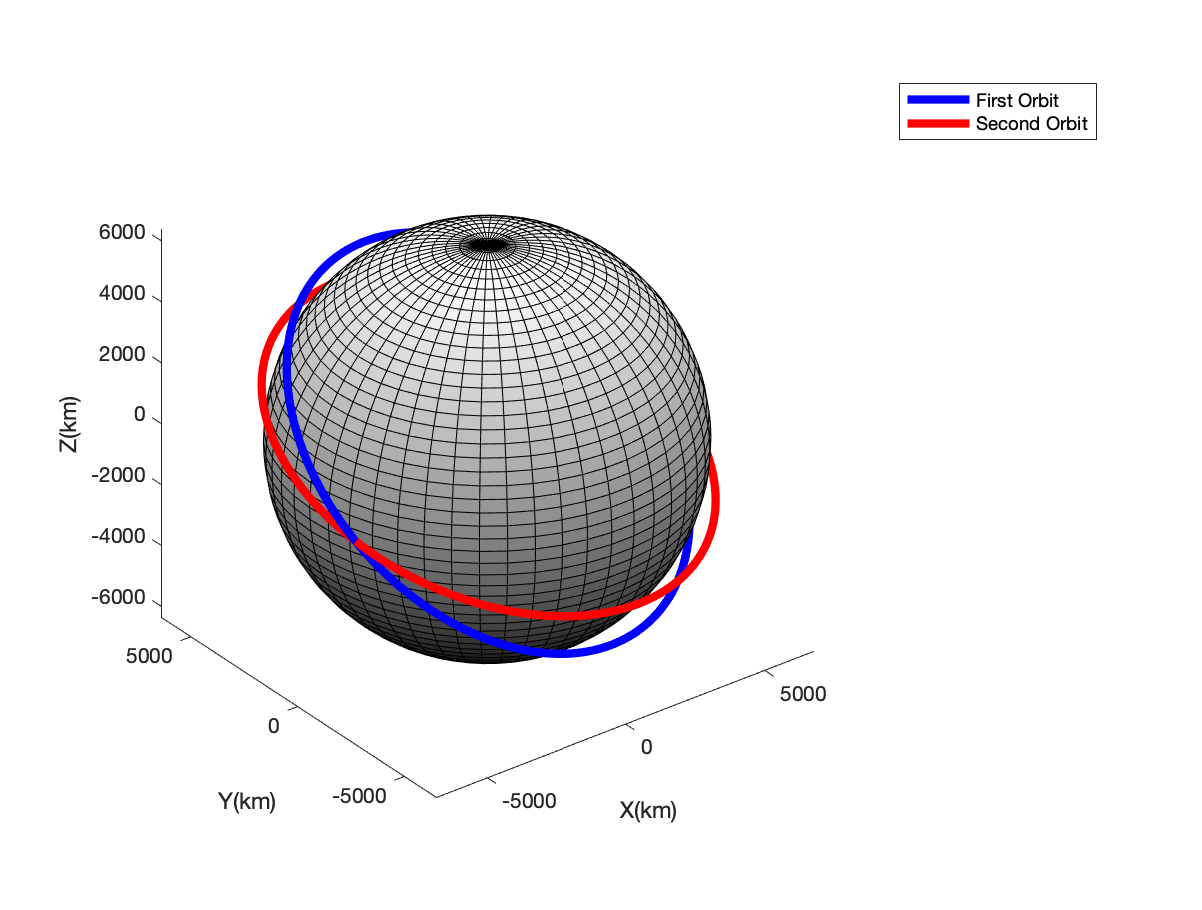
\includegraphics[width=16cm]{../Figure/Q2/3Dof_view_compare}
\end{figure}

\begin{figure}[H]
    \caption{3D trajectory in zx axis}
    \centering
    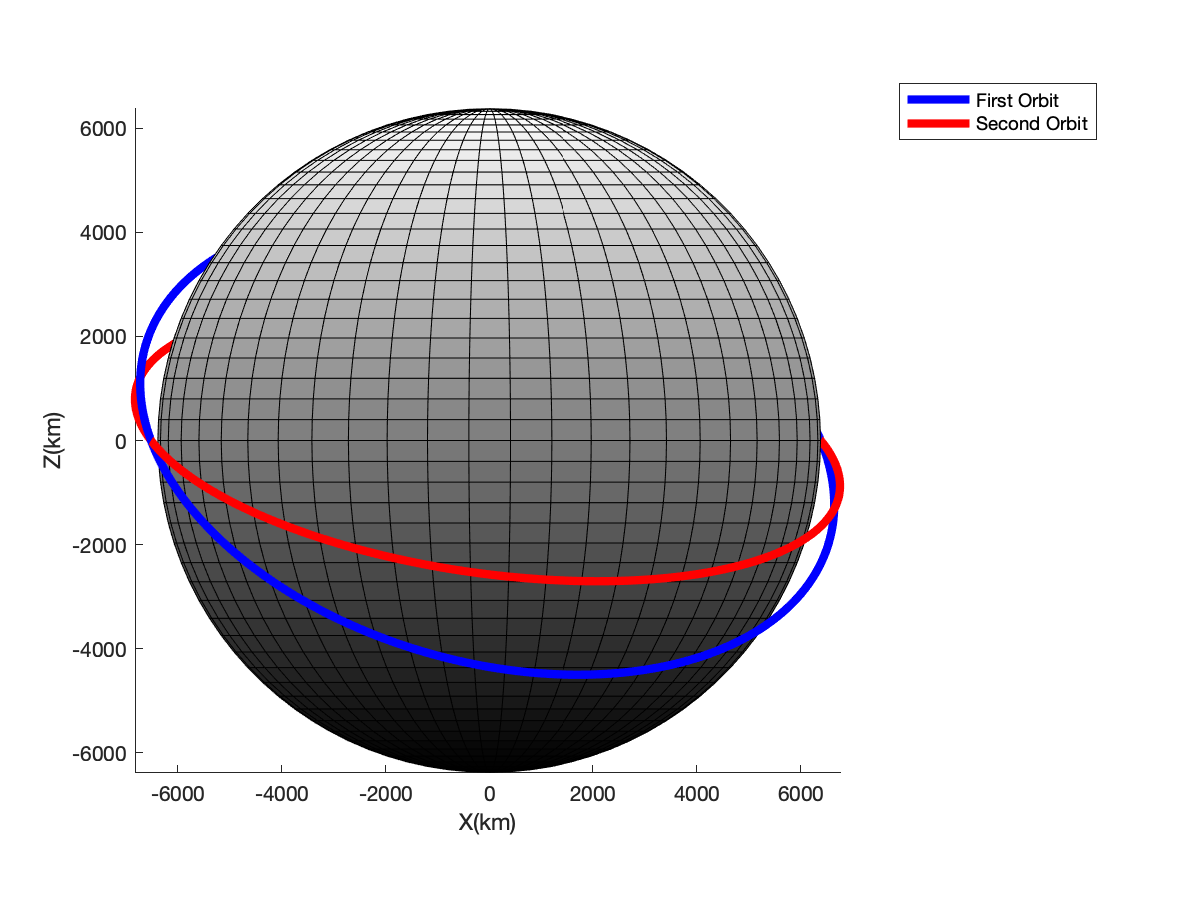
\includegraphics[width=16cm]{../Figure/Q2/xz_view_compare}
\end{figure}

\begin{figure}[H]
    \caption{3D trajectory in zy axis}
    \centering
    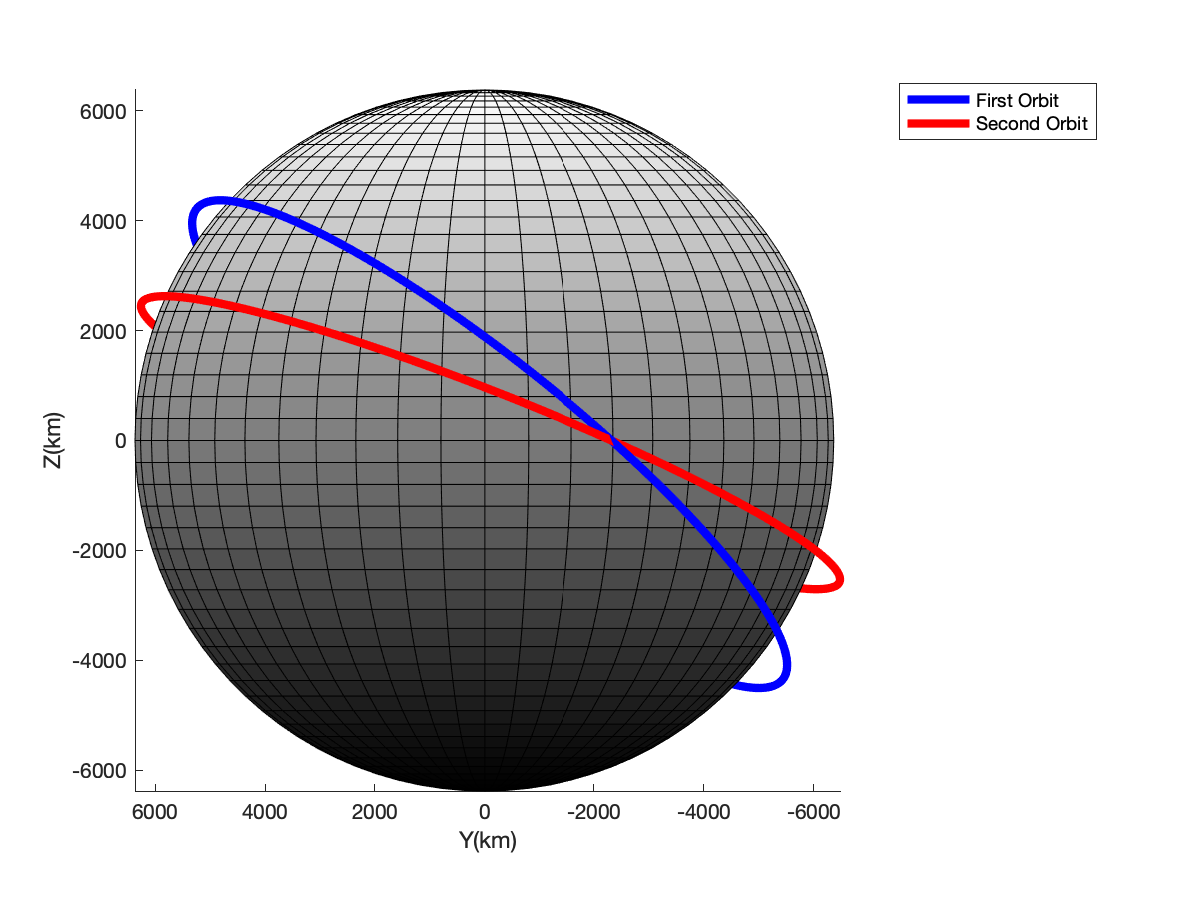
\includegraphics[width=16cm]{../Figure/Q2/yz_view_compare}
\end{figure}

\begin{figure}[H]
    \caption{3D trajectory in xy axis}
    \centering
    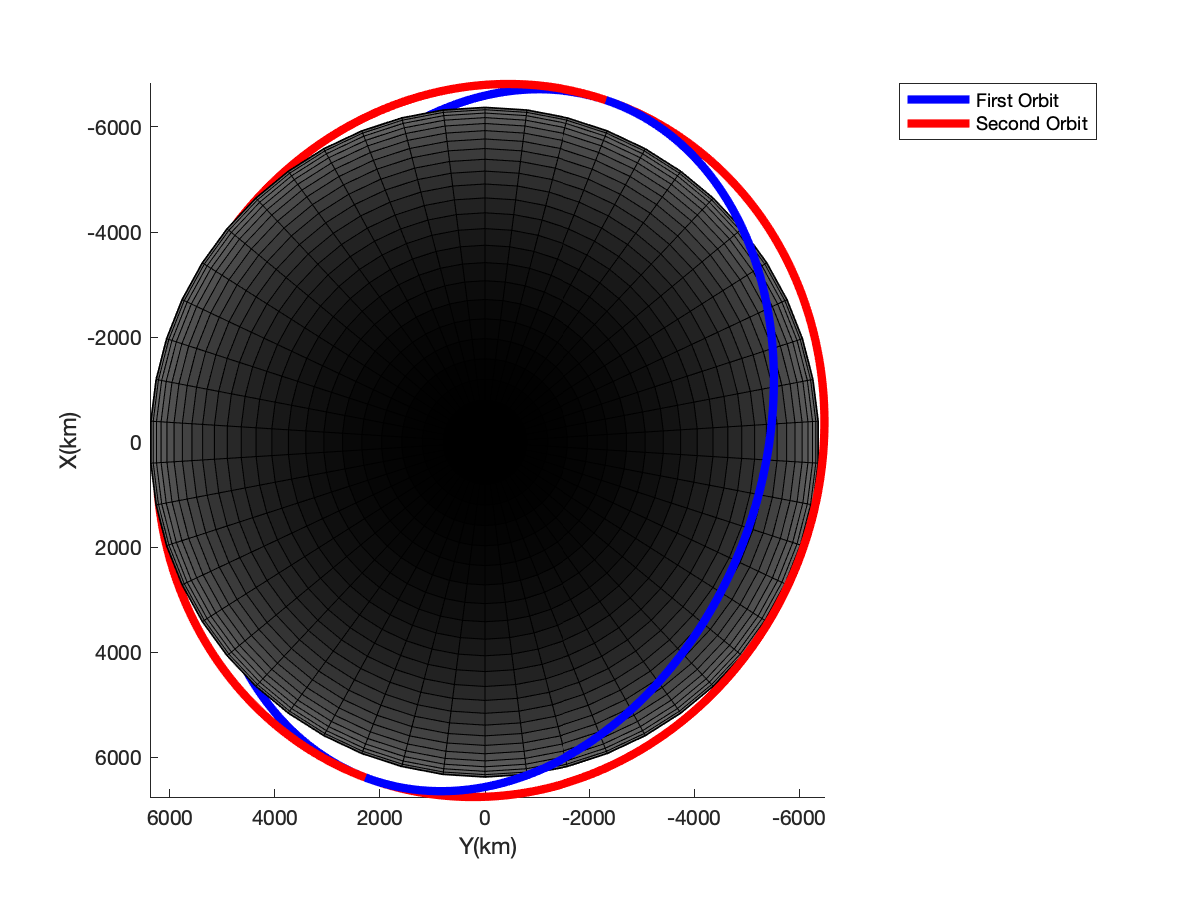
\includegraphics[width=16cm]{../Figure/Q2/xy_view_compare}
\end{figure}

\begin{figure}[H]
    \caption{Satellite latitude versus its longitude for one day}
    \centering
    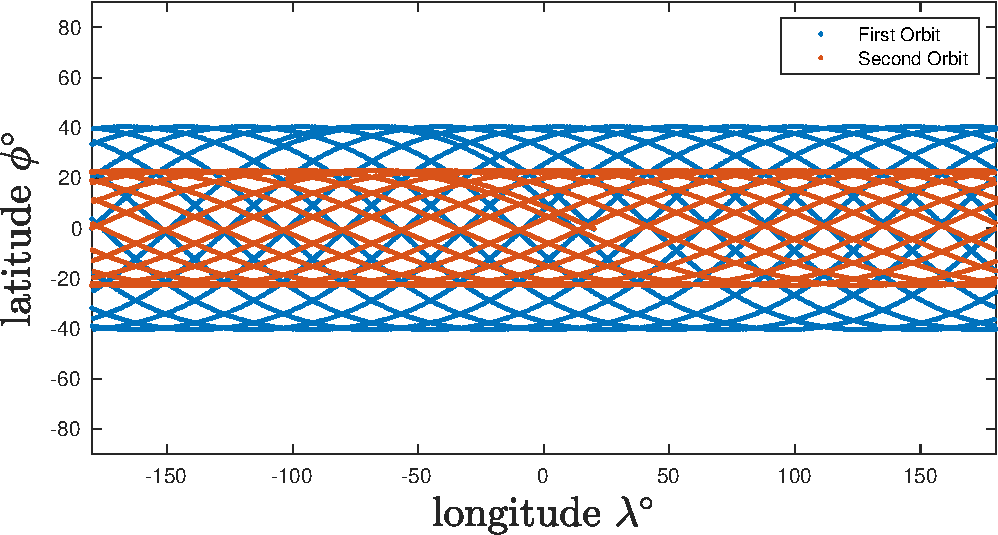
\includegraphics[width=16cm]{../Figure/Q2/latlong_compare}
\end{figure}
In general, changing the inclination of a satellite's orbit will cause its ground track to move to different latitudes and longitudes on the Earth's surface. In this example when the inclination changed from $0.7_{rad}$ to $0.4_{rad}$, the range of longitude decreased.